\documentclass[11pt]{article}
\usepackage[margin=1in]{geometry}
\usepackage[T1]{fontenc}
\usepackage{lmodern,microtype,amsmath,amssymb,amsthm,booktabs,graphicx}
\usepackage{pgfplots}
\pgfplotsset{compat=1.18}
\usepackage[hidelinks]{hyperref}
\usepackage{natbib}
\setlength{\parskip}{3pt}
\widowpenalty=10000
\clubpenalty=10000
\newcommand{\ind}{\mathbf{1}}
\newcommand{\E}{\mathbb{E}}
\newcommand{\Var}{\operatorname{Var}}
\newcommand{\Cov}{\operatorname{Cov}}
\newcommand{\sgn}{\operatorname{sgn}}
\newtheorem{proposition}{Proposition}
\title{What snapshot sampling does to\ order flow imbalance}
\author{Brendan Connelly \and Rigel Mummers}
\date{October 22, 2026}
\begin{document}
\maketitle
\begin{abstract}
We study a measurement problem that arose while trying to reproduce order flow imbalance results with minute snapshots. Applying the usual quote-transition formula once to a block's endpoints generally differs from summing the transitions observed inside it. Across 483 US stocks, the two measures have opposite signs in 17.03\% of materially nonzero five-minute comparisons in 2019 (95\% interval: 16.82--17.24\%), rising to 21.61\% at thirty minutes. We derive the aggregation error and give a simple model in which both measures have the same high contemporaneous fit despite persistent sign disagreement. A frozen-queue control explains 54.32\% of five-minute return variation; bounding ordinary endpoint OFI raises its fit from 24.25\% to 49.88\%, an important qualification. Neither observed measure improves our controlled five-minute forward forecast. The evidence supports a measurement check alongside price-fit statistics, rather than a new trading claim. It does not identify the error relative to event-level OFI.
\end{abstract}
\noindent\textbf{Keywords:} order flow imbalance; limit order book; temporal aggregation; market microstructure; measurement.\\
\textbf{JEL classifications:} C43, C58, G14.

\section{Why we looked at this}
We wanted to know how much of the earlier evidence on order flow imbalance (OFI) we could reproduce with the data we actually had. Our archive contains order-book snapshots at one-minute intervals, mostly with one level and sometimes with ten. It therefore records quote states, not a complete sequence of orders, cancellations and executions. That distinction limits what a replication can establish before any forecasting model is fitted.

The construction in \citet{cks} adds signed contributions from individual book events. Once those contributions have been retained, aggregation over time is straightforward. A different operation is to discard the intermediate observations and apply the same quote-transition formula once to the endpoints of a longer interval. We examine that substitution. Both quantities can be called snapshot OFI, and both incorporate price changes, but they need not measure the same direction of pressure.

Our contribution is a paired empirical audit of this difference, together with an explicit explanation of why contemporaneous price fit does not validate the measurement. We compare the two constructions on the same observed paths and with the same normalization. We then separate three questions: whether their signs agree, whether they explain the current return, and whether they improve a subsequent-return forecast. Keeping these questions separate is useful even when the available observations cannot establish which construction better approximates event OFI.

This is not a new objection to incomplete order-book observations. \citet{su} discuss snapshot limitations and develop generalized OFI to accommodate price changes across multiple ticks using deeper book information. Their work is the closest comparison. Our study does not implement that estimator, claim to improve it, or establish that snapshot OFI is intrinsically unusable. Instead, it quantifies the effect of replacing an already observed path by its endpoints. The formulas below are elementary consequences of the standard operator; we do not claim them as new general mathematical results.

The distinction also matters relative to other OFI research. \citet{xu} study multi-level OFI and contemporaneous price changes, while \citet{ccz} distinguish contemporaneous cross-impact from lagged predictive effects. Static queue imbalance can itself predict the next price move in a different setting \citep{gould}. Our one-minute, best-level comparison is neither a replication nor a refutation of those richer designs. Its narrower purpose is to make a potentially consequential change in measurement visible.

\section{What the endpoints leave out}
\subsection{Two constructions on one observed path}
Let $x_j=(b_j,q^b_j,a_j,q^a_j)$ be the best bid and ask prices and displayed sizes at observation $j$. Prices satisfy $0<b_j<a_j$, and sizes are positive. For one side of the book, define
\begin{equation}
 B(p_0,q_0;p_1,q_1)=q_1\ind\{p_1\geq p_0\}-q_0\ind\{p_1\leq p_0\}.
 \label{eq:B}
\end{equation}
Writing $B^b_j=B(b_{j-1},q^b_{j-1};b_j,q^b_j)$ and $B^a_j=B(-a_{j-1},q^a_{j-1};-a_j,q^a_j)$, the usual signed contribution is $e_j=B^b_j-B^a_j$. Reversing ask prices gives the standard ask-side convention: a falling ask contributes negative pressure.

For a block of $n$ observed transitions, let $D_0=(q^b_0+q^a_0)/2$. We compare
\begin{equation}
 F_n=\frac{\sum_{j=1}^{n}e_j}{D_0},\qquad
 C_n=\frac{B(b_0,q^b_0;b_n,q^b_n)-B(-a_0,q^a_0;-a_n,q^a_n)}{D_0}.
 \label{eq:FC}
\end{equation}
$F_n$ retains the observed minute transitions; $C_n$ retains only the block endpoints. We call them the minute sum and endpoint contribution. Neither is event-level OFI. Using a common positive denominator isolates the effect of discarding observations. Summing separately normalized minute contributions would define another statistic and would mix aggregation with changing weights.

\begin{proposition}[Exact aggregation error]
For any observed one-sided path, define
\begin{align}
 E^B={}&\sum_{j=1}^{n}\left(q_{j-1}\ind\{p_j>p_{j-1}\}-q_j\ind\{p_j<p_{j-1}\}\right)\nonumber\\
 &-q_0\ind\{p_n>p_0\}+q_n\ind\{p_n<p_0\}.
 \label{eq:error}
\end{align}
Then the sum of its transition contributions minus its endpoint contribution equals $E^B$. Applying this expression to bid prices and to negative ask prices gives $F_n-C_n=(E^b-E^a)/D_0$.
\end{proposition}
\begin{proof}
Checking increasing, decreasing and unchanged prices in \eqref{eq:B} gives
\[
 B(p_{j-1},q_{j-1};p_j,q_j)
 =q_j-q_{j-1}+q_{j-1}\ind\{p_j>p_{j-1}\}-q_j\ind\{p_j<p_{j-1}\}.
\]
Summing telescopes the size differences to $q_n-q_0$. Subtracting the same expression applied once to the endpoints cancels that term and leaves \eqref{eq:error}. Subtract the reversed-ask identity from the bid identity and divide by $D_0$.
\end{proof}

Flat price paths have zero aggregation error even when sizes change. Monotone paths need not: several upward bid transitions count several queues, whereas the endpoint calculation counts only the last queue. Thus reversals are one source of disagreement, but they are not necessary for a difference in magnitude.

\begin{proposition}[Endpoint ambiguity]
Endpoint states alone do not identify the sum of observed contributions over unrestricted valid quote paths. With constant bid size $q>0$, there are two paths with the same endpoints whose unnormalized net contributions are $+q$ and $-q$. Any endpoint-only estimate has absolute error at least $q$ on one of them.
\end{proposition}
\begin{proof}
For $\delta>0$ and $p>2\delta$, take the bid-price paths
\[
 (p,p+\delta,p+2\delta,p)\quad\text{and}\quad(p,p-\delta,p-2\delta,p).
\]
Keep bid size $q$, and hold a positive ask size and an ask price above $p+2\delta$ fixed. These are noncrossed paths. Their bid contributions are $(q,q,-q)$ and $(-q,-q,q)$, and their ask contributions are zero. Both endpoint contributions vanish. For any common endpoint estimate $u$, the triangle inequality gives $2q\leq |u-q|+|u+q|$, so the larger error is at least $q$.
\end{proof}
Repeating either closed path $k$ times gives a lower bound $kq$ when the number of intermediate observations is unrestricted. This is a deterministic ambiguity statement, not a bound for a fixed five-minute grid or a claim about conditional mean error. Additional path assumptions, deeper observations or a stochastic model can still support useful estimators.

\subsection{Equal explanatory fit does not resolve the ambiguity}
A simple model shows why comparing contemporaneous $R^2$ is not enough. Let minute log returns $X_j$ be independent $N(0,\sigma^2)$ with $\sigma>0$. Let the midpoint follow the corresponding positive geometric random walk, with bid and ask equal to $(1-s)$ and $(1+s)$ times the midpoint for fixed $0<s<1$. Keep both displayed sizes equal to $q>0$. Set $R_n=\sum_j X_j$.

\begin{proposition}[Fit and sign disagreement can coexist]
In this model, $F_n=2\sum_j\sgn(X_j)$ and $C_n=2\sgn(R_n)$. Both have population contemporaneous OLS $R^2=2/\pi$ for every $n$, but
\begin{equation}
 \lim_{n\to\infty}\Pr\{F_nC_n<0\}
 =\frac{\arccos\sqrt{2/\pi}}{\pi}\simeq 0.20595.
 \label{eq:null}
\end{equation}
Both have zero population covariance with an independent following-block return.
\end{proposition}
\begin{proof}
Each upward price transition contributes $2q$ and each downward transition $-2q$, giving the stated features after division by $D_0=q$. Symmetry gives zero means. With $S_n=\sum_j\sgn(X_j)$,
\[
 \Cov(R_n,S_n)=n\E|X_1|,\quad \Var(R_n)=n\sigma^2,\quad \Var(S_n)=n.
\]
Since $\E|X_1|=\sigma\sqrt{2/\pi}$, their squared correlation is $2/\pi$. For the endpoint feature, $R_n$ is Gaussian and
\[
 \operatorname{Corr}^2(R_n,\sgn R_n)
 =\frac{(\E|R_n|)^2}{\E R_n^2}=\frac{2}{\pi}.
\]
The joint central limit theorem for $(R_n/(\sigma\sqrt n),S_n/\sqrt n)$ gives a standard bivariate normal limit with correlation $\rho=\sqrt{2/\pi}$. Its opposite-sign probability is $\arccos(\rho)/\pi$, yielding \eqref{eq:null}; the quadrant boundary has zero limiting probability. Independence and zero mean give the final covariance statement.
\end{proof}

For even finite $n$, $F_n$ can be zero; that probability vanishes in the limit. Our simulations report ties separately and condition finite-sample disagreement on nonzero features. With 100,000 simulated paths and 1,001 increments, disagreement is 20.52\%, and both empirical $R^2$ values are approximately 63.75\%.

This model deliberately retains price changes in the features. It is not a model of actual order arrival, an equilibrium with no trading, or evidence that real order flow is irrelevant. It establishes only that high, equal explanatory fit can coexist with different measured directions. A diagnostic based on fit alone cannot rule out that possibility.

\section{Data and empirical design}
\subsection{Observed sample and measurement estimand}
The archive contains 483 US stocks selected by 2017 coverage, with available minute observations through 2019. Of these, 378 have one-level source files and 105 have ten-level files. We use only the best level for all stocks. The primary five-minute comparison contains 25,475,162 valid blocks across 358,807 stock-days. Blocks do not overlap, begin at 10:00 and end by 15:55. Shortened and exceptional sessions were excluded upstream. An additional 135 candidate blocks fail the within-block quote or extreme-return checks. We require positive prices and sizes, an uncrossed book throughout each block, and absolute within-block log return below 0.2.

We compare one-, two-, five-, ten- and thirty-minute grids, as well as a five-minute grid shifted by two minutes. The one-minute comparison is an identity check: the two constructions use the same single transition. Larger scales discard increasingly many observed states, but none supplies information between the original minute snapshots.

A comparison is \emph{material} when both $|F_n|$ and $|C_n|$ exceed $\tau=0.1$ starting-depth units. For stock $i$, date $d$, and eligible blocks $w$, define
\begin{equation}
 p_{id}(\tau)=\frac{\sum_w\ind\{|F_{idw}|>\tau,|C_{idw}|>\tau,F_{idw}C_{idw}<0\}}
 {\sum_w\ind\{|F_{idw}|>\tau,|C_{idw}|>\tau\}}.
 \label{eq:rate}
\end{equation}
We average $p_{id}$ equally across stocks within a date, omitting stock-days with a zero denominator, and then equally across dates. This estimand describes a typical stock-day, rather than allowing the number of surviving observations to set the weights. We also report pooled counts to make the conditioning transparent.

Intervals use 2,000 circular moving-block bootstrap draws of dates, with block length 20 trading days and seed 279. Resampling dates jointly across stocks preserves their observed contemporaneous dependence; consecutive dates within a block retain short-range temporal dependence. It does not establish independence beyond that scale or account for research choices made after looking at the archive. We examine block lengths 10 and 40 as descriptive sensitivity checks.

\subsection{Explanatory and forward models}
For each stock and scale, we fit ridge regressions on 2017, select the penalty from $\{0.01,1\}$ using 2018, refit through 2018 and evaluate in 2019. Training observations determine feature clipping at the 0.001 and 0.999 quantiles and subsequent standardization. Each same-block model has one feature: $F_n$, $C_n$, or a frozen-size endpoint control
\begin{equation}
 Z_n=\frac{q^b_0\sgn(b_n-b_0)+q^a_0\sgn(a_n-a_0)}{D_0}.
 \label{eq:frozen}
\end{equation}
This removes within-block size changes but retains the observed price moves. It is therefore an explanatory control, not an independently observed flow variable.

The forward target is the midpoint log return over the following block. The baseline uses the current and previous block returns, endpoint spread, log depth and queue imbalance, and trailing five- and thirty-minute returns. We add either $F_n$ or $C_n$ to that baseline. Predictors are observed by the current block's endpoint; target-path validity is an eligibility filter, not a predictor. Paired comparisons use identical eligible windows. The current-return models and next-return models answer different questions, even though their fitting chronology is the same.

Let $L_m$ denote model $m$'s mean squared error, first averaged within each stock-day, then equally across stocks within dates and across dates. Let $L_0$ use the corresponding stock's training-period mean return. We report
\begin{equation}
 R_m^2=1-L_m/L_0,\qquad G_{m:r}=1-L_m/L_r,
 \label{eq:loss}
\end{equation}
where $G_{m:r}$ is the relative MSE gain against reference $r$. These are ratios of aggregated losses, not averages of stock-specific $R^2$ values. Bootstrap draws recompute the ratios using jointly resampled dates. Four primary five-minute contrasts receive Holm correction: endpoint versus minute sum, frozen versus endpoint, and each forward addition versus baseline.

After observing the raw explanatory comparison, we added fixed $\tanh$ and sign transforms. The $\tanh$ scale is one, not a tuned value. We report all five variants and treat these comparisons, including the paired frozen-versus-bounded contrast, as post-result descriptive checks. The chronological split reduces fitting leakage, but these years were already examined in earlier project work. It does not make 2019 an untouched research holdout.

\section{Results}
\subsection{Direction changes under endpoint substitution}
Table~\ref{tab:scale} reports material sign disagreement in 2019. At five minutes, the estimate is 17.03\% (95\% interval: 16.82--17.24\%). The material filter retains 95.91\% of valid windows: 1,377,269 of 8,091,184 retained comparisons have opposite signs. Their pooled ratio differs slightly from the equal-stock, equal-day estimate in \eqref{eq:rate}. Disagreement increases to 21.61\% at thirty minutes.
\begin{table}[htbp]
\centering
\caption{Material sign disagreement by aggregation scale, 2019. Both absolute measures must exceed 0.1. Intervals resample dates jointly across stocks in 20-day blocks.}
\label{tab:scale}
\begin{tabular}{rrr}
\toprule Block length (minutes)& Opposite signs (\%) &95\% interval (\%)\\\midrule
1&0.00&[0.00, 0.00]\\
2&11.79&[11.51, 12.09]\\
5&17.03&[16.82, 17.24]\\
10&19.49&[19.28, 19.68]\\
30&21.61&[21.36, 21.87]\\\bottomrule
\end{tabular}
\end{table}

The five-minute estimate is 15.98\% in 2017 and 17.08\% in 2018. Moving the grid two minutes gives 17.27\% in 2019. All 483 stock-level rates in 2019 are positive; their median is 17.64\%, with 10th and 90th percentiles of 13.56\% and 19.59\%. The one-level and ten-level source groups have rates of 16.77\% and 17.97\%, respectively. Because both groups are measured at level one and contain different stocks, that difference is not an effect of observing more depth.

The result is also insensitive to the small-flow cutoff and the reported bootstrap alternatives. At cutoffs 0.001 and 0.01, five-minute disagreement is 17.91\% and 17.80\%. For the primary cutoff, changing the bootstrap block length to 10 or 40 days gives intervals of 16.87--17.22\% and 16.79--17.26\%. These checks do not turn an exploratory study into a confirmatory one, but they make a near-zero-flow or single-grid explanation less plausible.

\subsection{High fit is compatible with different measurements}
Table~\ref{tab:fit} compares five-minute explanatory fit. The untransformed minute sum and endpoint contribution explain 23.38\% and 24.25\% of test-period variation. The frozen-size control explains 54.32\%. Read alone, that gap could encourage a strong interpretation about the information in queue-size changes. The transformation results substantially qualify it: $\tanh(C_n)$ explains 49.88\%, and $\sgn(C_n)$ explains 48.72\%.
\begin{table}[htbp]
\centering
\caption{Same-block explanatory fit at five minutes, 2019. Values are $R^2$ in percent. The lower panel was added after inspecting the upper-panel results. None of these rows is a forward forecast.}
\label{tab:fit}
\begin{tabular}{lrr}
\toprule Feature&$R^2$&95\% interval\\\midrule
Minute sum $F_n$&23.38&[21.23, 25.22]\\
Endpoint $C_n$&24.25&[22.19, 25.97]\\
Frozen-size endpoint $Z_n$&54.32&[53.28, 55.49]\\\midrule
$\tanh(F_n)$&37.45&[36.66, 38.38]\\
$\tanh(C_n)$&49.88&[48.84, 51.05]\\
$\sgn(F_n)$&32.31&[31.61, 33.12]\\
$\sgn(C_n)$&48.72&[47.69, 49.88]\\
$\sgn(R_n)$, outcome-based diagnostic&52.49&[51.46, 53.67]\\\bottomrule
\end{tabular}
\end{table}

Bounding endpoint OFI closes much of the raw fit gap. The frozen-size control still has 8.86\% lower MSE than $\tanh(C_n)$ (descriptive 95\% interval: 8.52--9.20\%) on 8,436,055 matched windows. But this residual difference also compares distinct nonlinear functions of observed quotes. It is not a causal estimate of the role of queue updates. Likewise, the return-sign feature intentionally contains the outcome and is only a diagnostic benchmark. Its 52.49\% fit illustrates why a price-containing feature can explain a large share of current returns without being a useful forecast.

Figure~\ref{fig:comparison} puts the two parts of the evidence together. Endpoint substitution changes direction frequently, while a bounded endpoint feature can fit current returns well. The point is not that one $R^2$ is too high. It is that explanatory fit and agreement between measurements are different properties.
\begin{figure}[htbp]
\centering
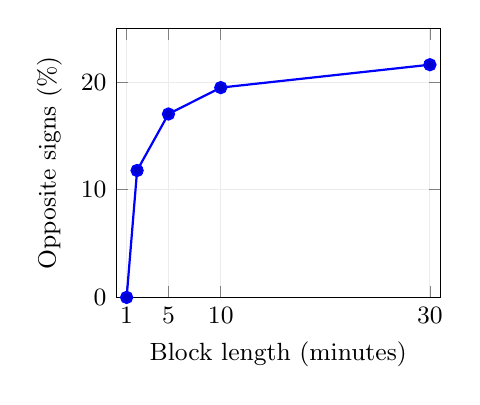
\begin{tikzpicture}
\begin{axis}[width=.47\textwidth,height=5cm,xlabel={Block length (minutes)},ylabel={Opposite signs (\%)},xmin=0,xmax=31,ymin=0,ymax=25,xtick={1,5,10,30},grid=major,grid style={gray!15},tick label style={font=\small},label style={font=\small}]
\addplot+[mark=*,thick,error bars/.cd,y dir=both,y explicit] coordinates {(1,0) +- (0,0) (2,11.7868) +- (0,.29) (5,17.0320) +- (0,.21) (10,19.4855) +- (0,.20) (30,21.6113) +- (0,.26)};
\end{axis}
\end{tikzpicture}\hfill
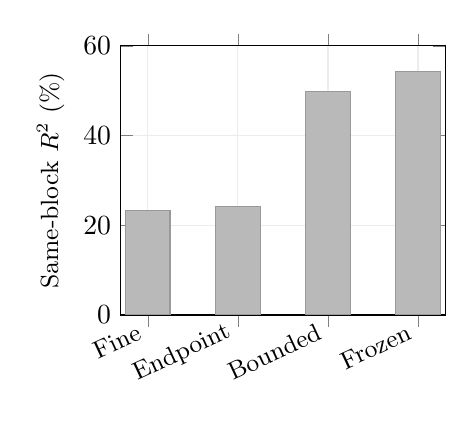
\begin{tikzpicture}
\begin{axis}[width=.47\textwidth,height=5cm,ybar,bar width=16pt,ylabel={Same-block $R^2$ (\%)},ymin=0,ymax=60,symbolic x coords={Fine,Endpoint,Bounded,Frozen},xtick=data,x tick label style={rotate=25,anchor=east,font=\small},label style={font=\small},grid=major,grid style={gray!15}]
\addplot[fill=gray!55,draw=gray!80] coordinates {(Fine,23.3816) (Endpoint,24.2527) (Bounded,49.8805) (Frozen,54.3219)};
\end{axis}
\end{tikzpicture}
\caption{Measurement disagreement and explanatory fit, 2019. Left: material disagreement; small error bars show approximately symmetric 95\% intervals (exact bounds in Table~\ref{tab:scale}). Right: five-minute fit, including the post-result bounded endpoint check. The minute sum is a finer observed reference, not event-level ground truth.}
\label{fig:comparison}
\end{figure}

\subsection{The forward comparison is much smaller}
The five-minute baseline has test-period $R^2=0.0778\%$. Adding the minute sum or endpoint contribution gives 0.0732\% and 0.0742\%, respectively. Relative to baseline, their MSE increases by 0.0046\% and 0.0036\%. The corresponding relative-gain intervals are $[-0.0066,-0.0029]\%$ and $[-0.0053,-0.0021]\%$. Both changes are precisely estimated but economically tiny. Neither addition provides a positive gain; the four primary loss contrasts retain significance under the reported Holm adjustment.

We do not infer that OFI never predicts returns, that all nonlinear models would fail, or that event-level and cross-asset signals are absent. This test concerns two own-stock snapshot features, a specified baseline and the following five-minute return. It supports keeping the contemporaneous measurement result separate from a claim about trading value. No transaction-cost or execution claim follows from these regressions.

\section{Preservation and implementation checks}
A practical way to avoid the additional loss is to retain additive contributions before coarsening the data. For each chunk, save summed bid and reversed-ask increments, boundary timestamps and quote states, and any additive quantities needed for normalization. Adjacent summaries merge by addition after checking their shared boundary. A depth sum and increment count permit normalization by mean depth; retaining the starting quote permits the starting-depth normalization used here. These denominators should not be silently interchanged.

Our implementation checks contiguous observation times and matching boundary states, rejects gaps, and counts each transition once. It reproduces direct aggregation and associative merging. This is ordinary additive aggregation applied to the observed operator, not a new compression method. It protects information already recorded; it cannot recover events missed between the finest snapshots.

We checked numerical precision because sign comparisons are sensitive near zero. Cached sizes are reconstructed from float32 log-depth and imbalance. In an audit of 18 original stock-day files spanning six stocks and all three years, four exact zero flows became tiny nonzero cached values. The largest sampled normalized five-minute flow error was 0.000122. This motivated reporting thresholds of 0.001, 0.01 and 0.1 rather than relying on an almost-zero cutoff. The audit is a selected sample check, not a universal numerical error bound.

Across eligible blocks, the largest normalized residual in the aggregation identity was $4.86\times10^{-11}$ or less. We independently replayed 210 saved models against 7,560 stock-day losses, with maximum MSE difference below $3.4\times10^{-21}$. All 17 relevant implementation and statistical tests pass. These checks support the stated calculations; they cannot correct selection in the source archive, supply missing event data, or establish novelty.

\section{Discussion and conclusion}
We find a substantial difference between two constructions that can otherwise look like interchangeable implementations of snapshot OFI. In the primary comparison, endpoint substitution changes the sign in about one in six material five-minute windows. The effect is present across years, grid phases and stocks, and becomes larger on the coarser grids considered. A high contemporaneous $R^2$ does not make that measurement difference disappear.

The claim is deliberately limited. The minute sum is not ground truth for event OFI. It can itself miss changes between snapshots, and this study does not establish that it is a better forecasting feature. Nor does it establish that endpoint constructions in earlier studies were implemented incorrectly. The relevant warning is conditional: when a researcher substitutes one endpoint transition for a sum of retained transitions, that substitution changes the measured variable and should be checked directly.

Several limitations remain. The archive may have survivorship and coverage selection, and a three-year US-equity sample need not represent other markets or regimes. Different depth normalizations or path restrictions may change the comparison. Our stock grouping is observational, not a controlled depth experiment. The fitting chronology does not eliminate the effects of earlier research on these years, and the bounded transformations were introduced after the raw fit comparison. Restricted access to the underlying archive also limits independent reproduction of the empirical estimates.

The closest unresolved comparison is generalized snapshot OFI \citep{su}. A common-data benchmark would help determine whether the present audit adds a useful diagnostic beyond existing measurement corrections. We cannot supply that comparison by treating the one-level archive as if it contained deeper events. A separate event-level sample could test how both observed constructions relate to fully observed contributions, but that is a different empirical question from the paired loss of information documented here.

Our conclusion is that a snapshot OFI study should report what was retained before aggregation, check its construction at more than one resolution, and distinguish current-price explanation from forward prediction. The evidence here makes that recommendation concrete. It supports a measurement note; it does not establish a new profitable signal or, by itself, settle whether the combination is sufficiently distinct for publication.

\paragraph{Reproducibility and data availability.}
Code, specifications, aggregate tables, tests and verification records are available in the project's research branch: \url{https://github.com/RM1505/math279_project/tree/research/ofi-snapshot-study-2026/replication_2026}. The underlying minute quote archive is not redistributed. The repository therefore permits inspection of the calculations and rerunning of synthetic checks, but full empirical reproduction requires access to the source data. The manuscript is a research draft pending coauthor review. AI assistance was used in analysis code, verification and drafting; this statement does not imply that all authors have approved the current version.

\begin{thebibliography}{9}
\bibitem[Cont et~al.(2014)]{cks} Cont, R., Kukanov, A., and Stoikov, S. (2014). The price impact of order book events. \emph{Journal of Financial Econometrics}, 12(1), 47--88. \href{https://doi.org/10.1093/jjfinec/nbt003}{doi:10.1093/jjfinec/nbt003}.
\bibitem[Cont et~al.(2023)]{ccz} Cont, R., Cucuringu, M., and Zhang, C. (2023). Cross-impact of order flow imbalance in equity markets. \emph{Quantitative Finance}. Author manuscript: \href{https://arxiv.org/abs/2112.13213}{arXiv:2112.13213}.
\bibitem[Gould and Bonart(2015)]{gould} Gould, M. D., and Bonart, J. (2015). Queue imbalance as a one-tick-ahead price predictor in a limit order book. \href{https://arxiv.org/abs/1512.03492}{arXiv:1512.03492}.
\bibitem[Su et~al.(2021)]{su} Su, Y., Sun, Z., Li, J., and Yuan, X. (2021). The price impact of generalized order flow imbalance. \href{https://arxiv.org/abs/2112.02947}{arXiv:2112.02947}.
\bibitem[Xu et~al.(2019)]{xu} Xu, K., Gould, M. D., and Howison, S. D. (2019). Multi-level order-flow imbalance in a limit order book. \href{https://arxiv.org/abs/1907.06230}{arXiv:1907.06230}.
\end{thebibliography}
\end{document}
